\documentclass[12pt]{report}

\usepackage[T1]{fontenc}
\usepackage[utf8]{inputenc}
\usepackage{graphicx}

\begin{document}
{\Large Los arreglos y parametros de los Amplificadores Clase B}\\
\Large{Enesto Alonso Partida López\\ Universidad Politecnica De La Zona Metropolitana De Guadalajara\\ Mecatronica 4 A\\ Septiembre-diciembre 2019}\\
{8 de octubre 2019 }\\


\includegraphics[scale=1]{../../../Downloads/upzmg.jpg} \\


\newpage
{\huge \textbf{¿Qué es un Amplificador de tipo B?}\\}

{\Large Se les denomina amplificador clase B, cuando el voltaje de polarización y la máxima amplitud de la señal entrante poseen valores que hacen que la corriente de salida circule durante el semiciclo de la señal de entrada.}\\
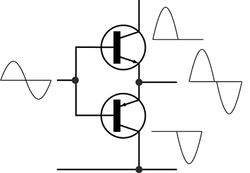
\includegraphics[scale=1]{../../../Downloads/descragas/1.png}  

{\huge \textbf{¿Comó se clasifican los amplificadores?}\\}\\


{\Large Se clasifican principalmente por la frecuencia con la que estos trabajan, asi se conocen las clase A, B, AB y C las cuales tiene difentes usos y aplicaciones, ademas,estos se dividen en amplificadores de potencia y tensión, en este caso solo nos centraremos en los Amplificadores de tipo A}\\



{\huge \textbf{Amplificador de tensión y potencia}\\}\\


{\Large Los aplificadores de tension son aquellos que suministran una mayor tension en su salida, cuando su tension de entrada es menor. Por otro lado tenemos los aplificadores de potencia los cuales al igual que los de tension, su tension es mayor en la salida que en la entrada, pero a demas, su corriente es mucho mayor en la salida que en la entrada. Por eso su nombre de amplificadores de potencia }\\
\\
{\huge \textbf{Funcionamiento de un amplificador de potencia  }\\}\\

{\Large Un amplificador de potencia funciona en clase A cuando la tensión de polarización y la amplitud máxima de la señal de entrada poseen valores tales que hacen que la corriente de salida circule durante todo el período de la señal de entrada.  Y la diferncia que tiene con un amplificador de tipo B es que el amplificador clase B su corriente de salida circula durante un semiperíodo de la señal de entrada.\\ En los amplificadores nunca existira una corrinete de reja(base.}\\
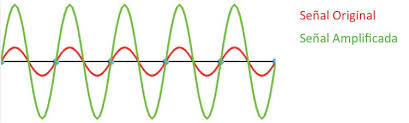
\includegraphics[scale=1]{../../../Downloads/descragas/3.jpg} \\

{\huge \textbf{Ventaja y desventaje de los amplificadores clase }\\}\\


{\Large \textbf{Sus principales ventajas}\\Posee bajo consumo en reposo.
Aprovecha al máximo la Corriente entregada por la fuente.
Intensidad casi nula cuando está en reposo.\\\\ \textbf{Sus principales desvenatjas}\\Producen armónicos, y es mayor cuando no tienen los transistores de salida con las mismas características técnicas, debido a esto se les suele polarizar de forma que se les introduce una pequeña polarización directa. Con esto se consigue desplazar las curvas y se disminuye dicha distorsión.\\\\ \textbf{Aplicaciones}\\ Sistemas telefónicos,
Transmisores de seguridad portátiles
Sistemas de aviso, aunque no en audio.}\\
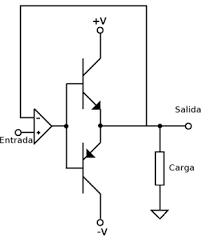
\includegraphics[scale=1]{../../../Downloads/descragas/2.png} 

\newpage
{\huge \textbf{Bibliografia:}\\}\\
{\large
@online{Electronica Unicrom,
author = {Luis González López},
title = {Amplificadores de Potencia: clasificación, clase A, B, AB, C},
year = {2016},
url = {https://unicrom.com/amplificadores-de-potencia-clasificacion/},
OPTsubtitle = {Amplificadores clase A},
OPTlanguage = {Español},
OPTversion = {1},
OPTdate = {21},
OPTmonth = {6},
OPTurldate = {https://unicrom.com/amplificadores-de-potencia-clasificacion/},
}
}

\end{document}